\documentclass[conference]{IEEEtran}
\IEEEoverridecommandlockouts
\usepackage{cite}
\usepackage{amsmath,amssymb,amsfonts}
\usepackage{algorithmic}
\usepackage{graphicx}
\usepackage{textcomp}
\usepackage{xcolor}
\usepackage{caption}
\usepackage{subcaption}
% \usepackage{natbib}

\begin{document}

\makeatletter
\newcommand{\linebreakand}{
  \end{@IEEEauthorhalign}
  \hfill\mbox{}\par
  \mbox{}\hfill\begin{@IEEEauthorhalign}
}
\makeatother

\title{Control de plataforma móvil de cuatro ruedas mecanum con modelo cinemático}

\author{
  \IEEEauthorblockN{
    1\textsuperscript{st}  Martinez, Brayan Steven
  }
  \IEEEauthorblockA{
    \textit{Ingeniería Mecatrónica} \\
    \textit{Universidad EIA}\\
    Medellín, Colombia \\
    brayan.martinez@eia.edu.co
  }
  \and
  \IEEEauthorblockN{
    2\textsuperscript{nd} Gongora, Juan Pablo
  }
  \IEEEauthorblockA{
    \textit{Ingeniería Mecatrónica} \\
    \textit{Universidad EIA}\\
    Medellín, Colombia \\
    juan.gongora@eia.edu.co
  }
  \and
  \IEEEauthorblockN{
    3\textsuperscript{rd} Isaza, Luis Miguel
  }
  \IEEEauthorblockA{
    \textit{Ingeniería Mecatrónica} \\
    \textit{Universidad EIA}\\
    Medellín, Colombia \\
    luis.isaza@eia.edu.co
  }
  \and
  \IEEEauthorblockN{
    4\textsuperscript{th} Jiménez, Sebastian David
  }
  \IEEEauthorblockA{
    \textit{Ingeniería Mecatrónica} \\
    \textit{Universidad EIA}\\
    Medellín, Colombia \\
    sebastian.jimenez10@eia.edu.co
  }
  \and
  \IEEEauthorblockN{
    5\textsuperscript{th} aaa, aaaa aaaa
  }
  \IEEEauthorblockA{
    \textit{Ingeniería Mecatrónica} \\
    \textit{Universidad EIA}\\
    Medellín, Colombia \\
    email
  }
}
\maketitle

\begin{abstract}
  El movimiento de plataformas móviles está compuesto de estrategias de control,
  modelos matemáticos que describen el movimiento del mismo, planificación de trayectorias y
  planificación de tareas, además de sensores que deben complementarse para lograr el
  objetivo deseado.
\end{abstract}

\begin{IEEEkeywords}
  robotica, trayectoria, cinemática, navegación
\end{IEEEkeywords}

\section{Introducción}
  Se presentan las simulaciones asociadas a un modelo cinemático para un robot omnidireccional 
  con cuatro ruedas estilo mecanum teniendo de cuenta los parámetros dimensionales del robot,
  más no, los análisis eléctricos o de leyes de control aplicables, se da una posible ruta
  para continuar con el trabajo a fin de contribuir a la construcción de un robot de
  servicio.
\section{Materiales y método}
\subsection{Materiales}
\textbf{Matlab} para realizar matemática computacional, programación de algoritmos y
gráficos a partir de los resultados.

\textbf{CoppeliaSim} para llevar a cabo simulaciones en un entorno virtual teniendo a
disposición robots predeterminador, sensores y un API para conectarse con otros
lenguajes de programación.

\textbf{Odroid-XU4} como tarjeta de desarrollo para ser implementada de forma
tentativa en el robot. Características de buen rendimiento y tamaño la convierten
en una opción para integrar todos los sistemas.

\textbf{ROS (Robot Operating System)} como framework para complementar varios
sistemas en uno solo y permitir una fluida comunicación entre los mismo. Se instala
sobre una distribución de Linux.

\textbf{Ubuntu} como sistema operativo para implementar en el robot aprovechando
las ventajas de ROS y la compatibiliadd con sistemas de desarrollo como la
ODROID-XU4 y sensores.

\textbf{Modelo cinemático} \cite{noauthor_modelo_nodate} para predecir el comportamiento de la plataforma que
posee cuatro ruedas suecas (mecanum)

\textbf{Plataforma móvil} con cuatro motores y ruedas suecas (mecanum), la configuración
para este trabajo es como sigue en la Figura \ref{fig:platformmec}.

\begin{figure}
  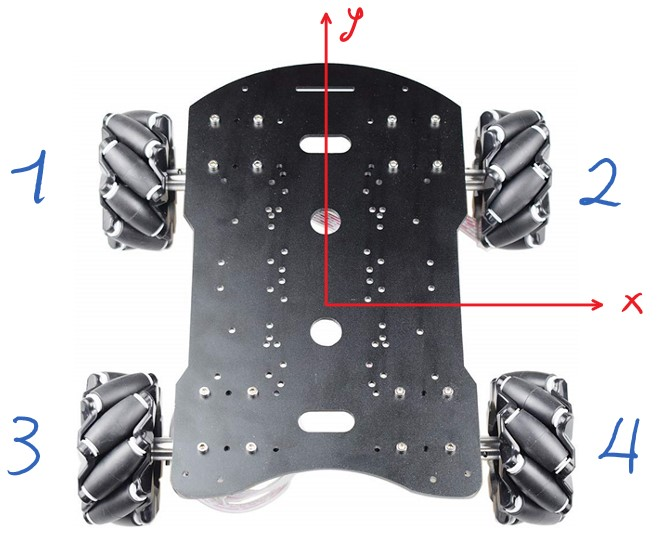
\includegraphics[width=\linewidth]{figures/plataforma_config.jpg}
  \caption{Plataforma mecánica con motores y ruedas}
  \label{fig:platformmec}
\end{figure}

\subsection{Método}
\subsubsection{Simulación Matlab}
Se analiza el modelo cinemático ya conocido:
\begin{gather}
  \begin{bmatrix} \omega_{1} \\ \omega_{2} \\ \omega_{3} \\ \omega_{4} \end{bmatrix}
  =
  \frac{1}{r}
  \begin{bmatrix}
    1  & 1 & -(L+l) \\
    -1 & 1 & (L+l)  \\
    -1 & 1 & -(L+l) \\
    1  & 1 & (L+l)
  \end{bmatrix}
  \begin{bmatrix} V_{s} \\ V_{y} \\ \omega \end{bmatrix}
\end{gather}

\begin{figure}
  \centering
  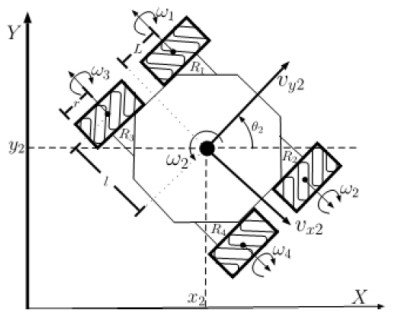
\includegraphics[width=0.8\linewidth]{figures/omnidirectional_robot.jpg}
  \caption{Robot omnidireccional a modelar}
  \label{fig:omnirobot}
\end{figure}

En base a la Figura \ref{fig:omnirobot}, Los parametros L, l y r, pertenecen 
al robot, para esta simulación, al KUKA YouBot \cite{noauthor_kuka_nodate},
donde: r = 100 mm, L = 235.5 mm, l = 150 mm.

A este modelo matemático se le ingresan las velocidades en X, Y y rotación angular
del robot, para obtener la velodiadad angular de cada rueda. Se programa la función 
que representa este modelo cinámatico en Matlab y además, otra función para convertir 
las posiciones deseadas en velocidad lineal usando las ecuaciones
\ref{vx}, \ref{vy} y \ref{omega} teniendo en cuenta una metodología de control por 
campos potenciales \cite{gonzalez-villela_cinematica_2015} 
visibles en la Figura \ref{fig:campospotenciales}

\begin{figure}
  \centering
  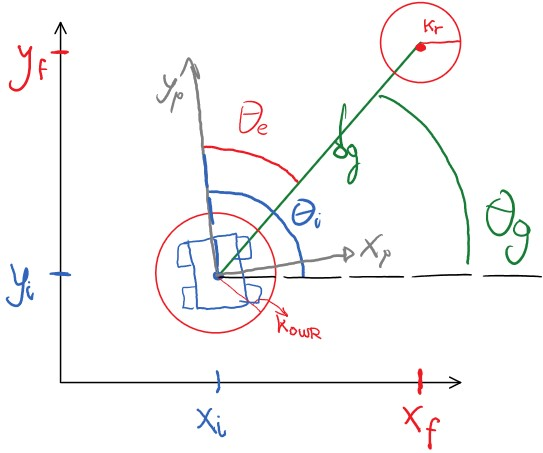
\includegraphics[width=0.9\linewidth]{figures/campos_potenciales.jpg}
  \caption{Robot en el plano con campos potenciales}
  \label{fig:campospotenciales}
\end{figure}

\begin{gather}\label{vy}
  V_{x}= \left\{ \begin{array}{lcc}
    Vx_{max} \sin \theta_{e} & si & d_{g} > K_{r}+K_{owr} \\
    \\ \frac{d_{g}}{K_{r}+K_{owr}} \sin \theta_{e} &  si & d_{g} \leq  K_{r}+K_{owr} \\
    \\ 0 &  si  & d_{g} = 0
  \end{array}
  \right.
\end{gather}

\begin{gather}\label{vx}
  V_{y}= \left\{ \begin{array}{lcc}
    Vx_{max} \cos \theta_{e} & si & d_{g} > K_{r}+K_{owr} \\
    \\ \frac{d_{g}}{K_{r}+K_{owr}} \cos \theta_{e} &  si & d_{g} \leq  K_{r}+K_{owr} \\
    \\ 0 &  si  & d_{g} = 0
  \end{array}
  \right.
\end{gather}

\begin{gather}\label{omega}
  \omega = \omega_{max}+\sin \theta_{e}
\end{gather}

Con las ecuaciones \ref{vx}, \ref{vy} y \ref{omega} se pueden obtener las velocidades
angulares de cada rueda gracias al modelo cinemático.

Observando la Figura \ref{fig:campospotenciales} se nota que es necesario en todo
momento conocer la posición actual del robot y así calcular los vectores y ángulos;
es fácil de obtener cuando hay otro sistema externo que proporciona esas coordenadas, pero,
para una simulación en Matlab, es necesario encontrar los nuevos valores cada que el objeto
se desplazada con las ecuaciones \ref{newx}, \ref{newy} y \ref{newt}, cuyas variables
se pueden observar en la Figura \ref{fig:newpositions}.

\begin{figure}
  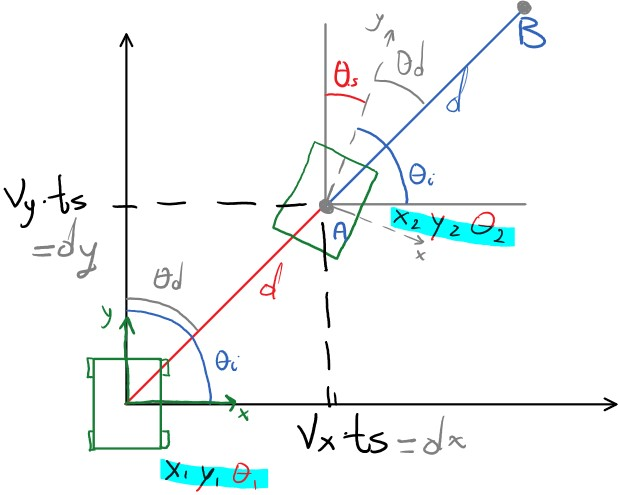
\includegraphics[width=\linewidth]{figures/new_positions.jpg}
  \caption{Desplazamiento del robot en el plano cartesiano}
  \label{fig:newpositions}
\end{figure}

\begin{gather}
  d = \sqrt{(d_{x})^2+(d_{y})^2}
\end{gather}

\begin{gather}
  d_{x} = V_{x} T_{s}
\end{gather}
\begin{gather}
  d_{y} = V_{y} T_{s}
\end{gather}

\begin{gather}
  \theta_{d} = \tan^{-1}\frac{d_{x}}{d_{y}}
\end{gather}

\begin{gather}\label{newx}
  x_{2} = x_{1} + 
        \left(
          d
          \sin
            \left(
              {\theta_{d} + \frac{\pi}{2} - \theta_{i} }
            \right)  
        \right) 
\end{gather}

\begin{gather}\label{newy}
  y_{2} = y_{1} + 
        \left(
          d
          \cos
            \left(
              {\theta_{d} + \frac{\pi}{2} - \theta_{i} }
            \right)  
        \right) 
\end{gather}

\begin{gather}\label{newt}
  \theta_{i_{2}} = \theta_{i_{1}} + \omega T_{s}
\end{gather}

Se recomienda ir al código para analizar la secuancia lógica.


\subsubsection{Simulación con CoppeliaSim}
Es necesario usar la API de CoppeliaSim en Matlab para llevar a cabo la simulación
aprovechano que ya se tiene el modelo cinemático programado y funcionando en Matlab.

Buscar los archivos del API en la ruta de CoppeliaSim :
"CoppeliaRobotics CoppeliaSimEdu programming remoteApiBindings matlab matlab",
para copiar únicamente los siguientes archivos en la carpeta con el main de Matlab para controlar el robot:
\begin{itemize}
  \item remApi
  \item remoteApiProto
  \item simpleText
\end{itemize}

En la misma carpeta, copiar otro archivo llamado remoteApi.dll que se encuentra en:
"CoppeliaRobotics CoppeliaSimEdu programming remoteApiBindings lib lib Windows"

El archivo 'simpleText' sirve como guía para usar el API con Matlab.

\section{Resultados}
\subsection{Simulación Matlab}
Se obtiene una primera simulación numérica usando Matlab.
El robot comienza en (0,0) a 90° de la horizontal, se desea que llegue a (1.5, 3.2).
El resultado se puede ver en la Figura \ref{fig:robotpos}. La orientación del robot
se va alineando con el vector definido por el punto inicial y final.

\begin{figure}
  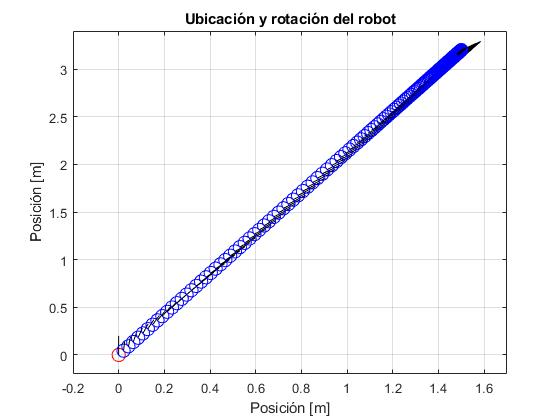
\includegraphics[width=\linewidth]{figures/matlab_pos_1.jpg}
  \caption{Registro de movimiento del robot}
  \label{fig:robotpos}
\end{figure}


Aprovechando el modelo cinemático, se puede graficar la velocidad angular de
los motores, como se observa en la Figura \ref{fig:motorang}, la velocidad se reduce hasta 0,
llegando así a la posición final.

\begin{figure}
  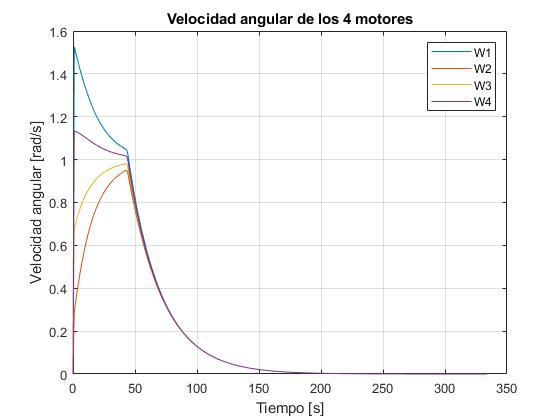
\includegraphics[width=\linewidth]{figures/matlab_motor_1.jpg}
  \caption{Velocidad angular de los motores en el tiempo}
  \label{fig:motorang}
\end{figure}

\subsection{Simulación CoppeliaSim}
Se obtiene también, una simulación virtual en base al modelo cinemático y un robot con el cual se prueba el modelo.
En CoppeliaSim se dispone del KUKA YouBot que viene por defecto, una plataforma con ruedas omnidireccionales.
\begin{figure}
  \centering
  \begin{subfigure}[b]{0.5\linewidth}
    \centering
    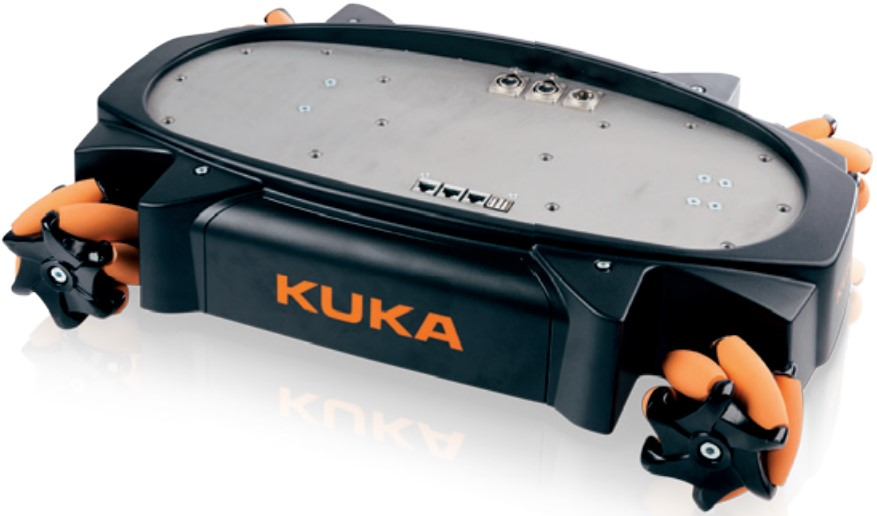
\includegraphics[width=\linewidth]{figures/kuka_real_youbot.jpg}
    \caption{En la realidad}
    \label{fig:kukayoubot}
  \end{subfigure}
  
  \begin{subfigure}[b]{0.5\linewidth}
    \centering
    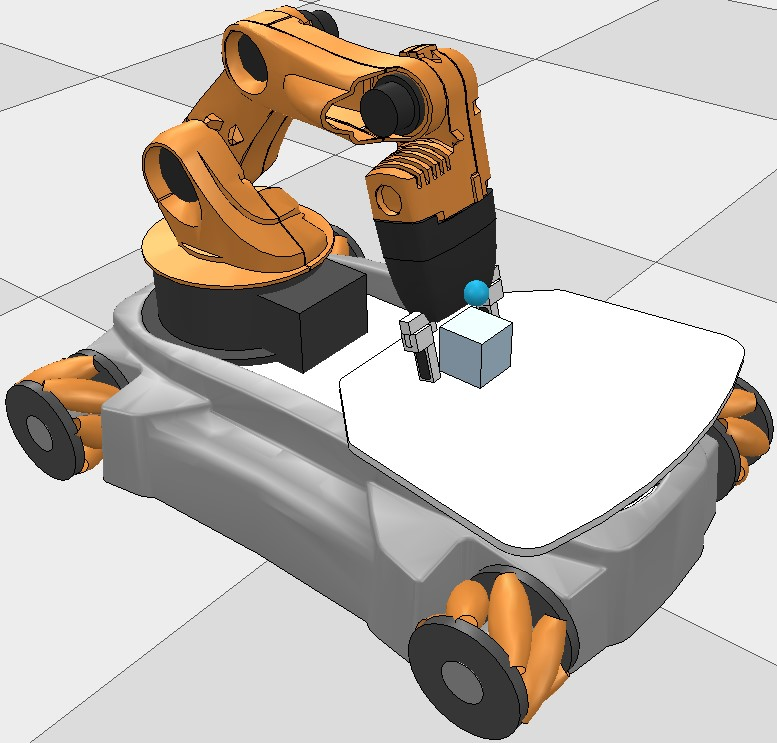
\includegraphics[width=\linewidth]{figures/kuka_sim_youbot.jpg}
    \caption{En CoppeliaSm}
    \label{fig:kukasimyoubot}
  \end{subfigure}
  \caption{KUKA YouBot}
\end{figure}

\begin{figure}
  \centering
  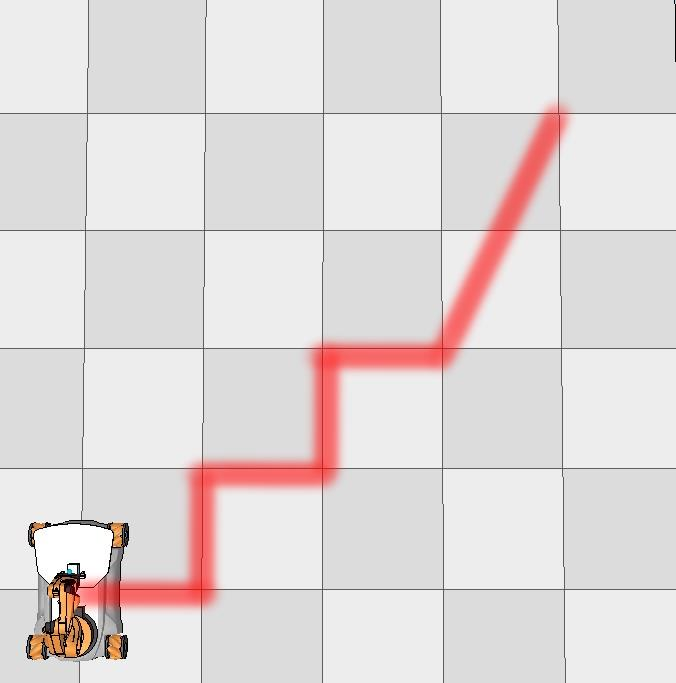
\includegraphics[width=0.6\linewidth]{figures/kuka_init_pos.jpg}
  \caption{Ruta programada para el KUKA YouBot y posición inicial}
  \label{fig:kukaroute}
\end{figure}

\begin{figure}
  \centering
  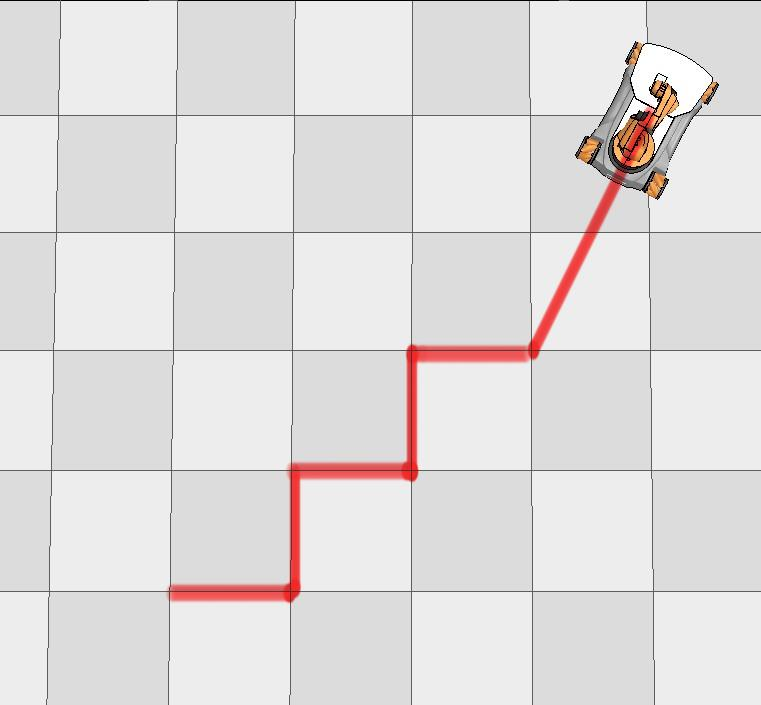
\includegraphics[width=0.6\linewidth]{figures/kuka_final_pos.jpg}
  \caption{Posición final KUKA YouBot}
  \label{fig:kukafinal}
\end{figure}

Se programó un desplazamiento como en la Figura \ref{fig:kukaroute} donde al final
se incluye una rotación y se puede visualizar en la Figura \ref{fig:kukafinal}.


Se conocen alternativas más cercanas al entorno real de implementación como
Gazebo\cite{noauthor_gazebo_nodate}, que no se logró probar para esta iteración del semillero; se sabe que se puede
complementar con ROS (Robot Operating System) y eso significa que se puede aprovechar
para elementos o dispositivos electrónicos físicos.

\subsection{Revisión Odroid}
Se instaló satisfactoriamente la distribución Ubuntu de Linux en sus versiones 16 y 18
sobre la tarjeta de desarrollo Odroid-XU4 presentando algunos problemas iniciales de
apagado indeseado cuando se le cargaba al sistema operativo con más procesos,
solucionable con una fuente de mejor calidad o también con un arreglo de diodo, capacitor
y resistencia para evitar los cortes súbitos pero momentáneos de energía.

\subsection{Aprendizajes en ROS}
En relación con el punto anterior, se logró instalar ROS (Robot Operating System)
sobre Ubuntu 16 y correr algunos de sus ejemplos predeterminados como la TurtleBot,
además, entender brevemente aunque sin profundizar, en la estructura de este sistema operativo.

\subsection{Cámara Orbbec Astra}
Se realizaron pruebas con la cámara de profunidad Orbbec Astra concluyendo que
es un excelente complemento para determinar el entorno tridimensional que rodea
al robot de servicio, este dispositivo permite conocer la profuncidad de cada punto
de la imagen, el programa se corre en Linux y la cámara es USB.

\subsection{LiDAR}
Se sabe de paquetes de ROS que son una gran alternativa para realizar mapeo con ROS como son:
\begin{itemize}
  \item Google Cartographer
  \item Hector Slam
\end{itemize}

\section{Discusión o análisis de resultados}
La simulacuón en CoppeliaSim no se pudo realizar más compleja porque los ángulos de rotación
entregados por el API a Matlab no son cartesianos.

La velocidad angular de cada motor corresponde efectivamente con el movimiento que debería
hacer el robot en la realidad.

El movimiento simulado en CoppeliaSim no tuvo ningun tipo de problema, además el fin de cada
trayectoria se veía suavizado gracias al enfoque de campos potenciales \cite{gonzalez-villela_cinematica_2015}.

El punto de inicio y el punto de final de una trayectoria definen un vector al cual el robot
se intenta alinear si se incluye una medida de error entre la horientación del robot y el mencionado vector.

En la simulación no es posible determinar el ángulo final de robor, no se implementó.

La ruta aproximada para continuar con el proyecto es, en consecuencia con lo que ya se vió,
formar un mapa virtual partiendo de los sensores como cámara de profunidad y LiDAR usando
técnicas de SLAM con el fin de ubicar el robot en un espacio real de trabajo y prescindir
del control desde Matlab para llevarlo a cabo desde la tarjeta de desarrollo; posteriormente,
mentiras en algoritmos de control para los motores y así generar el movimiento deseado.

El penúltimo bloque se compone de la navegación segura para el robot, la fundamental para
guardar su integridad y por último, gestión tareas de movimiento.

\section{Conclusión}
\begin{itemize}
  \item La simulación con Matlab y CoppeliaSim en conjunto es muy útil, dado que el 
  segundo tiene muchos robots, sensores y objetos para crear entornos de simulación, 
  además se aprovecha la potencia de Matlab para la computación sin programar el 
  childScript en CoppeliaSim que resulta ser poco práctico.
  \item Se valido de manera aceptable por medio de simulaciones que el modelo cinamático 
  es funcional.
  \item Se pueden combinar la cámara de profunidad con el LiDAR para obtener una representación
  más fiel del entorno que rodea el robot.
  \item Matlab es un buen comienzo para planear el algoritmo de control y luego migrarlo
  a alternativas más útiles con la actual aplicación Robótica, usar ROS desde etapas
  temprana si se tiene todo el hardware puede resultar provechoso.
  \item Las simulaciones son muy aceptables pero en la realidad también hay consideraciones
  mecánicas y eléctricas, los problemas realmente están en el hardware.
  \item Es muy importante elegir un algoritmo o ley de control adecuada para los motores de 
  la forma correcta, el fallo en la actuación de estos elementos compromete todo el robot.
  \item Es muy crítico obtener la posición absoluta del robot en un entorno,
  esta variable de posición es entrada del modelo cinemático, es por esto que se piensa en
  cámara de profunidad y/o LiDAR para tener un mapeo general donde el robot se pueda ubicar.
\end{itemize}
\newpage

\bibliography{references}
\bibliographystyle{IEEEtran}

\end{document}